%---------------------------------------------------------------------------
%	Packages
%---------------------------------------------------------------------------
\documentclass[twocolumn]{article}
\usepackage[bottom]{footmisc}
\usepackage[affil-it]{authblk}
\usepackage{amsmath}
\usepackage{setspace}
\usepackage{url}
\usepackage{amsthm}
\usepackage{tikz}
\usetikzlibrary{shapes.geometric, arrows}
\usetikzlibrary{decorations.pathreplacing}
\usetikzlibrary{calc}
\usepackage{pgfplots}
\usepgfplotslibrary{units}
\usepackage{indentfirst}
\usepackage{gensymb}
\pgfplotsset{compat=1.10}
\usepackage{amsmath}
\usepackage{braket}
\usepackage{tikz}
\usetikzlibrary{shapes.geometric, arrows}
\usetikzlibrary{decorations.pathreplacing}
\usetikzlibrary{decorations.pathmorphing}
\usetikzlibrary{decorations.markings}
\usepackage{pgfplots}
\usepackage{pgf}
\usepackage{fancyhdr}
\usepgfplotslibrary{units}
\pgfplotsset{compat=1.10}
\usepgfplotslibrary{units}
\usepackage{tkz-euclide}
\usetkzobj{all}
\usepackage{xcolor}
\usepackage{graphicx}
\usetikzlibrary{arrows.meta}
\tikzset{>=Stealth}
\tikzset{snake it/.style={decorate, decoration=snake}}
\graphicspath{{Figures/}}
%---------------------------------------------------------------------------
%	Header and footer
%---------------------------------------------------------------------------
\pagestyle{fancy}
\lhead{\small{Quantum Parameter Estimation Progress}}
\chead{\small{T.J. Larrechea}}
\rhead{\small{Colorado Mesa University}}
%---------------------------------------------------------------------------
%	Title and Author
%---------------------------------------------------------------------------
\title{\textbf{PHYS 482 Progress Report}}
\author{Taylor Larrechea\footnote{Electronic Address: \texttt{tjlarrechea@mavs.coloradomesa.edu.}} \\
    Colorado Mesa University \\
    Department of Physical and Environmental Sciences \\
    1100 North Avenue \\
    Grand Junction, CO 81501-3122}
\date{\today}
%---------------------------------------------------------------------------
%	Begin Document
%---------------------------------------------------------------------------
\begin{document}
\maketitle
%---------------------------------------------------------------------------
%	Abstract
%---------------------------------------------------------------------------
\begin{abstract}
Quantum parameter estimation, or metrology, is the method of which quantum mechanical systems are used as measuring devices to measure physical parameters. This paper discusses the progress made in researching metrology for undergraduate research at Colorado Mesa University.
\end{abstract}
%---------------------------------------------------------------------------
%	Introduction
%---------------------------------------------------------------------------
\section*{Introduction}
Quantum parameter estimation deals with estimating physical parameters by using quantum mechanical systems as measuring devices. These systems can be used to measure physical parameters such as the strength of a magnetic field. In previous studies, done particularly by Dr. David Collins, Professor of Physics at Colorado Mesa University, metrology has been studied to see if there are better approximation methods that exist. Particularly if using states such as entangled states enhance the estimation accuracy compared to other classical strategies \cite{D. Collins}. The research that is being reported in this article covers a similar question about how to improve estimation accuracy, particularly by using multiple states at once. Product states as well as entangled states are examined to address the question that has been brought to attention in this article.
%---------------------------------------------------------------------------
%	Conceptual Understanding
%---------------------------------------------------------------------------
\section*{Conceptual Understanding}
The beginning task was to first understand what the research that was being done in this article meant conceptually. For example, take a particle that is being sent into a magnetic field. A particle that resides in a specific state, usually denoted by $\ket{\psi}$, can be subjected to a measurement influenced by a physical parameter. After the measurement is taken on the particle we can repeat this process hundreds of times to learn more about the probabilities of getting a specific measurement. Quantum physics tells us that the resulting measurement can come out to be either $S_{n+}=\hbar/2$ or $S_{n-}=-\hbar/2$. Both of these results will eventually add up to have a probability of one depending upon the original orientation of the particle in the given state $\ket{\psi}$.

When these experiments are repeated several times, that is subjecting a particle to a measurement, we begin to have a better understanding of the probability of either obtaining $\hbar/2$ or $-\hbar/2$ from our measurement. Using quantum mechanics we can then begin to state certain things about the state itself such as the angle $\theta$ and the angle $\phi$ from their respective axis'. The angles can be seen in Figure 1.
%--------------------------------------------------
%	Figure 1
%--------------------------------------------------
\begin{figure}[htbp]
\begin{center}
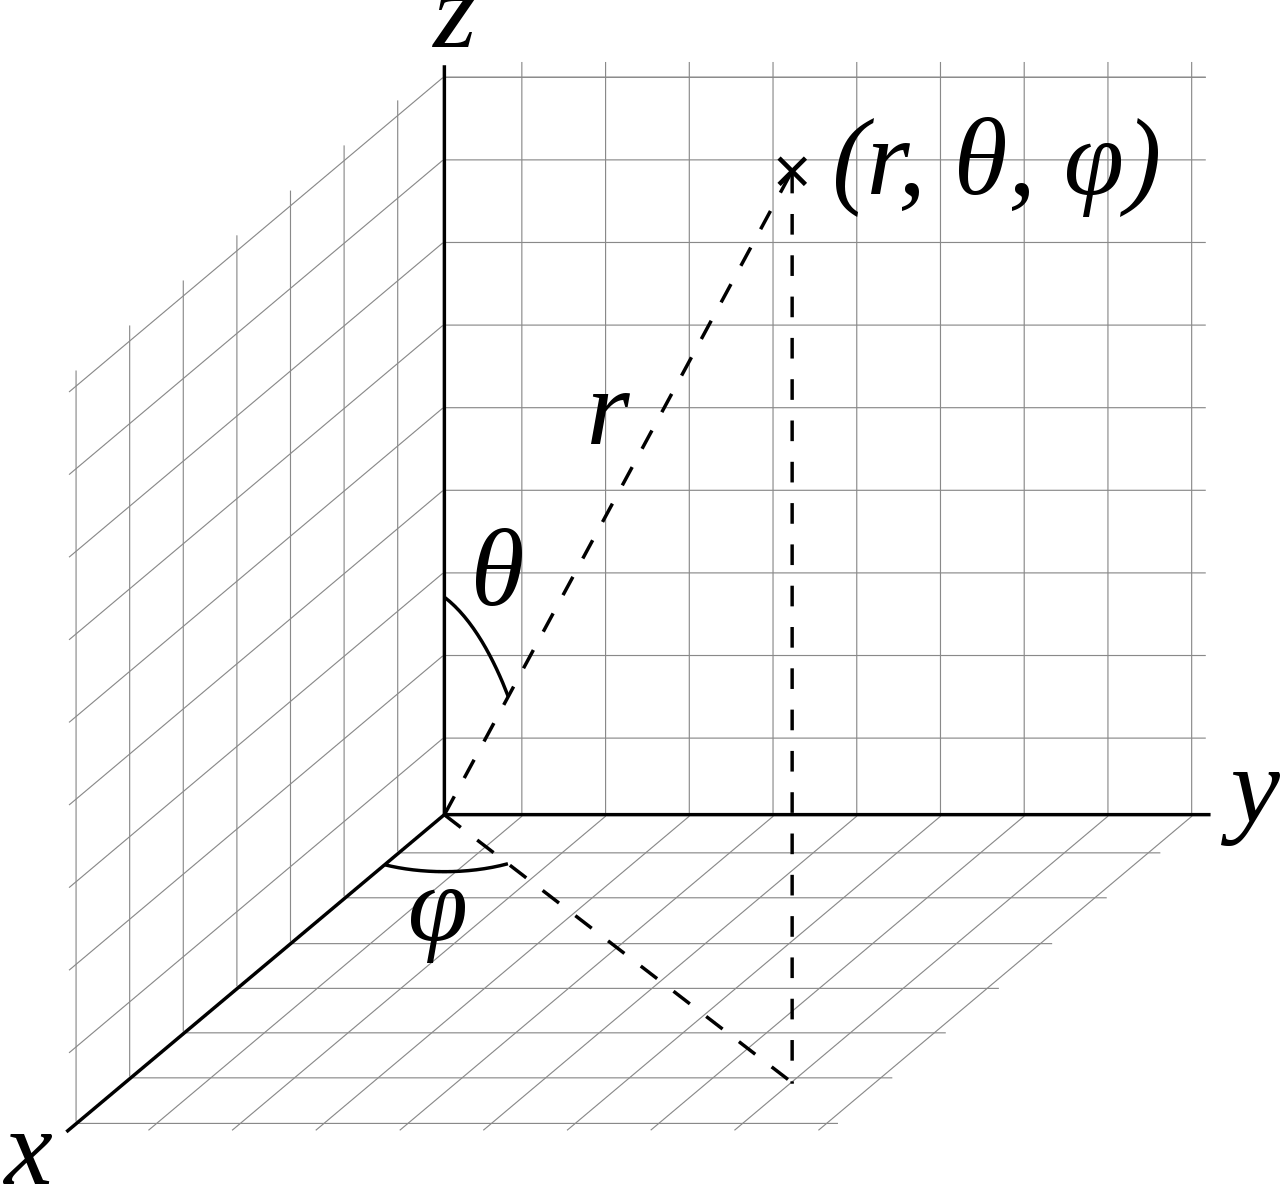
\includegraphics[width=0.75\linewidth]{Spherical-Coordinate-System.png}
\caption{Generic Representation of 3D Spherical Coordinate System.}
\end{center}
\end{figure}
\newline
\newline
Particles are subject to being measured can have any orientation with any value of $\theta$ or $\phi$. Typically these particles that are being described are spin - $1/2$ particles. We will now begin to discuss spin - $1/2$ particles that are present in a magnetic field.
%---------------------------------------------------------------------------
%	Classical Spin - 1/2 Paricles
%---------------------------------------------------------------------------
\section*{Classical Spin - $1/2$ Particles}
Spin - $1/2$ particles can exist in one of two states. The first state can be when these particles are considered to be ``positive" or orientated such that they are pointing above the x-y plane. The other state can be when these particles are ``negative" or orientated such that they are pointing below the x-y plane. Often one can read an academic article where the states of these particles are said to be ``noisy", which essentially means the collection of these particles are almost 50/50 in some being negative and others being positive.

When these particles are present within a magnetic field they have a tendency to ``flip". This flipping phenomenon is when the particles go from being in their positive to negative state or vice versa. For the sake of simplicity we will begin by taking a look at these particles that are present in a constant uniform magnetic field.
%--------------------------------------------------
%	Figure 2
%--------------------------------------------------
\begin{figure}[htbp]
\begin{center}
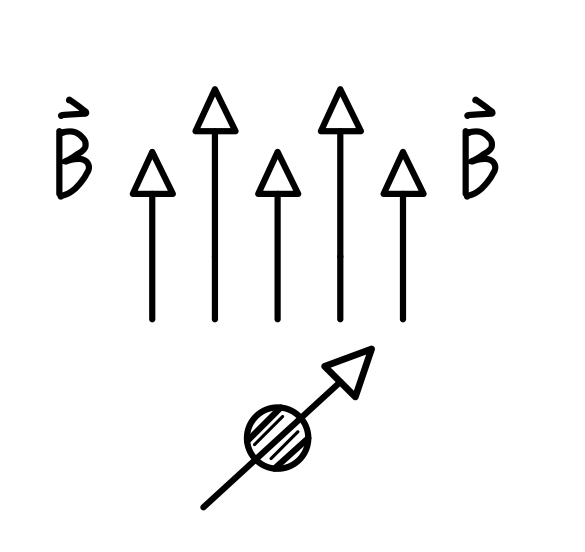
\includegraphics[width=0.75\linewidth]{Dipole-In-Magnetic-Field.PNG}
\caption{Dipole Present in a Magnetic Field.}
\end{center}
\end{figure}
\newline
Figure 2 is an artists rendition of a magnetic dipole that is in presence of a magnetic field. As the dipole is subjected to the magnetic field we should expect it to flip from one orientation to the other, this of course is dependent upon the initial orientation of the dipole. The torque that this dipole experiences can be calculated via
%--------------------------------------------------
%	Equation (1)
%--------------------------------------------------
\begin{equation}
\hat{\tau}=\hat{\mu} \times \hat{B}
\end{equation}
where $\hat{\mu}$ is the dipole moment and $\hat{B}$ is the magnetic field that it is experiencing. Using Isaac Newton's second law we can relate torque to
%--------------------------------------------------
%	Equation (2)
%--------------------------------------------------
\begin{equation}
\frac{d\hat{L}}{dt}=\hat{\tau}
\end{equation}
where $\hat{L}$ is the angular momentum of our particle. It turns out that $\hat{L}$ and $\hat{\mu}$ are proportional via
%--------------------------------------------------
%	Equation (3)
%--------------------------------------------------
\begin{equation}
\hat{L}=\frac{1}{\gamma}\hat{u}
\end{equation}
where $\gamma$ is dependent upon the situation that we are presented with. Finally we can represent the equation of motion for our dipole via
%--------------------------------------------------
%	Equation (4)
%--------------------------------------------------
\begin{equation}
\frac{d\hat{M}}{dt}=\gamma \hspace{2pt} (\hat{M} \times \hat{B})
\end{equation}
where $M=\Sigma \hspace{2pt} \hat{\mu}$. The next task is to solve equation (4) for each direction so that we can have a quantitative description of how our particle interacts with the magnetic field.
%---------------------------------------------------------------------------
%	Solving Equations of Emotion for Dipole
%---------------------------------------------------------------------------
\section*{Solving Equations of Emotion}
Equation (4) describes how we can measure magnetization of these spin - $1/2$ particles. There are three separate equations of emotion for the $x,\hspace{1pt}y,$ and $z$ directions. Those equations are
%--------------------------------------------------
%	Equation (5)
%--------------------------------------------------
\begin{equation}
\frac{dM_{x}}{dt}=\gamma(\hat{M}\times\hat{B})_{x}-\frac{M_{x}}{T_{2}},
\end{equation}
%--------------------------------------------------
%	Equation (6)
%--------------------------------------------------
\begin{equation}
\frac{dM_{y}}{dt}=\gamma(\hat{M}\times\hat{B})_{y}-\frac{M_{y}}{T_{2}},
\end{equation}
%--------------------------------------------------
%	Equation (7)
%--------------------------------------------------
\begin{equation}
\frac{dM_{z}}{dt}=\frac{M_{0}-M_{z}}{T_{1}}
\end{equation}
where $T_1$ and $T_2$ are parameters for a given situation. Equations (5) and (6) simplify significantly with the only magnetic field that is non zero is the $\hat{B}_z$. After separating variables and solving the differential equations the solutions to equations (5) and (6) are
%--------------------------------------------------
%	Equation (8)
%--------------------------------------------------
\begin{equation}
M_{x}=A\sin{(\gamma B_{z}t)}-B\cos{(\gamma B_{z}t)}
\end{equation}
%--------------------------------------------------
%	Equation (9)
%--------------------------------------------------
and
\begin{equation}
M_{y}=A\cos{(\gamma B_{z}t)}+B\sin{(\gamma B_{z}t)}.
\end{equation}
Equations (8) and (9) describe the rate at which the particles rotate in the $x-y$ plane classically. The solution to equation (7)
%--------------------------------------------------
%	Equation (10)
%--------------------------------------------------
\begin{equation}
M_{z}=M_{zi}e^{(-\frac{t}{T_1})}+M_{0}(1-e^{(-\frac{t}{T_1})})
\end{equation}
where equation (10) describes the rate of change that the spin - $1/2$ particle rotates from spin up ($+z$ orientation) to spin down ($-z$ orientation) or vice versa. Now that equations (5), (6), and (7) have been solved we can move on to examining these spin - $1/2$ in a different light.
%---------------------------------------------------------------------------
%	Quantum Spin - 1/2 Systems
%---------------------------------------------------------------------------
\section*{Quantum Spin - $1/2$ Systems}
There are ways that we can describe these spin - $1/2$ systems with the language of Quantum Mechanics. Conversely Quantum Mechanics can be described in the language of linear algebra, specifically in this case with bras and kets. These spin - $1/2$ systems can be described with the ket 
%--------------------------------------------------
%	Equation (11)
%--------------------------------------------------
\begin{equation}
\ket{\psi}=a_{+}\ket{+\hat{z}}+a_{-}\ket{-\hat{z}}
\end{equation}
where $a_{+}$ and $a_{-}$ are normalization constants. When we subject these particles to a measurement in either the $x, \hspace{1pt} y$, or $z$ direction we have the possibility of getting one of two outcomes. The two possible outcomes from this measurement are $+\hbar/2$ and $-\hbar/2$ and this scheme can be seen in Figure 3. \\
%--------------------------------------------------
%	Figure 3
%--------------------------------------------------
\begin{figure}[htpb]
\begin{center}
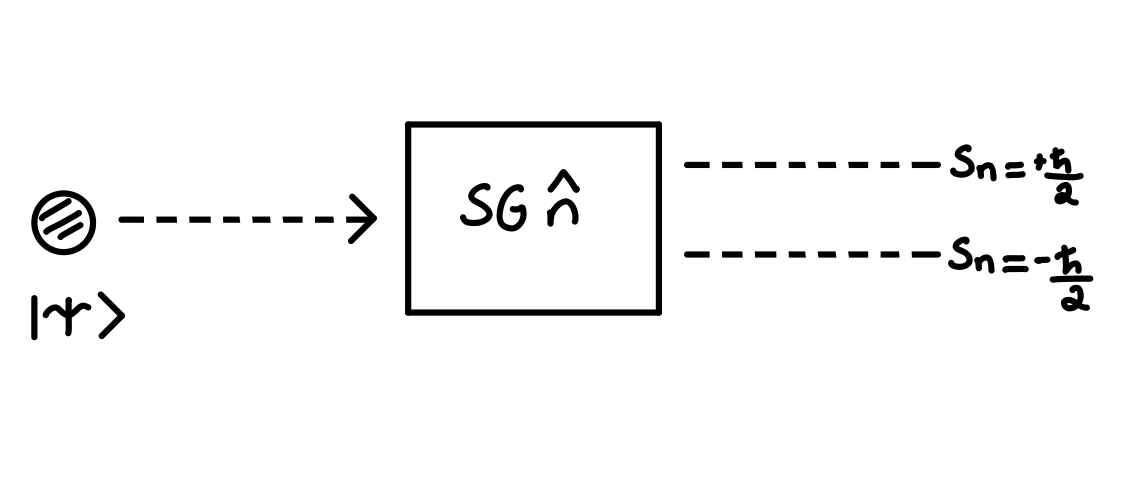
\includegraphics[width=0.90\linewidth]{SG-Measurement.PNG}
\caption{Artistic Rendition of SG Measurement.}
\end{center}
\end{figure}
\newline
Figure 3 encompasses a generic state $\hat{n}$ which can either be the $x, \hspace{1pt} y$, or $z$ direction. These states can represent the $x, \hspace{1pt} y$, or $z$ direction by knowing $\theta$ and $\phi$ for whatever particle we are interested in measuring. These states can be calculated by
%--------------------------------------------------
%	Equations (12)
%--------------------------------------------------
\begin{equation}
\ket{+\hat{n}}=\cos{(\theta/2)}\ket{+\hat{z}}+e^{i\phi}\sin{(\theta/2)}\ket{-\hat{z}}
\end{equation}
and
%--------------------------------------------------
%	Equations (13)
%--------------------------------------------------
\begin{equation}
\ket{-\hat{n}}=\sin{(\theta/2)}\ket{+\hat{z}}-e^{i\phi}\cos{(\theta/2)}\ket{-\hat{z}}.
\end{equation}
Once these states are known we can also calculate the probabilities of getting $+\hbar/2$ and $-\hbar/2$ by
%--------------------------------------------------
%	Equation (14)
%--------------------------------------------------
\begin{equation}
\text{Prob}=|\bra{\pm\hat{n}}\ket{\psi}|^2
\end{equation}
where the probabilities of getting $+\hbar/2$ and $-\hbar/2$ must add up to be 1.

It is more conventional to write equations (12) and (13) as in $\ket{0}$ and $\ket{1}$ notation. Precisely, these equations are
%--------------------------------------------------
%	Equation (15)
%--------------------------------------------------
\begin{equation}
\ket{+\hat{n}}=\cos{(\theta/2)}\ket{0}+e^{i\phi}\sin{(\theta/2)}\ket{1}
\end{equation}
and
%--------------------------------------------------
%	Equation (16)
%--------------------------------------------------
\begin{equation}
\ket{-\hat{n}}=\sin{(\theta/2)}\ket{0}-e^{i\phi}\cos{(\theta/2)}\ket{1}.
\end{equation}
The notation that is denoted in equation (15) and (16) is what will be used throughout the rest of this paper to described spin-1/2 particles with specific initial conditions.
%---------------------------------------------------------------------------
%	Entangled and Product States
%---------------------------------------------------------------------------
\section*{Entangled and Product States}
We continue our investigation into spin - 1/2 particles by examining entangled and product states. In short, entangled states and product states are states that involve multiple states. Product states are two states of which that can be separated into two separate individual states. Entangled states are states that involve two states that cannot be separated such that each individual state can be recognized.

Take for instance the state
%--------------------------------------------------
%	Equation (17)
%--------------------------------------------------
\begin{equation}
\ket{\psi}=\frac{1}{2}\big(\ket{0}\ket{0}+\ket{0}\ket{1}-\ket{1}\ket{0}-\ket{1}\ket{1}\big)
\end{equation}
which for instance is an example of a product state. Equation (17) can be written as a combination of states such that
%--------------------------------------------------
%	Equation (18)
%--------------------------------------------------
\begin{equation}
\ket{\psi}=\ket{\psi_A}\ket{\psi_B}.
\end{equation}
Precisely $\ket{\psi_A}$ can be written as
%--------------------------------------------------
%	Equation (19)
%--------------------------------------------------
\begin{equation}
\ket{\psi_A}=\frac{-1}{\sqrt{2}}\ket{0}+\frac{1}{\sqrt{2}}\ket{1}
\end{equation}
and $\ket{\psi_B}$ can be written as
%--------------------------------------------------
%	Equation (20)
%--------------------------------------------------
\begin{equation}
\ket{\psi_B}=\frac{-1}{\sqrt{2}}\ket{0}-\frac{1}{\sqrt{2}}\ket{1}.
\end{equation}
When equation (19) and (20) are multiplied together equation (17) is produced. Similar to single states, product and entangled states can have probabilities calculated. These probabilities are typically more complicated than single states but the mathematics of how these probabilities are calculated are the same. In general the formula for calculating probabilities in entangled and product states is
%--------------------------------------------------
%	Equation (21)
%--------------------------------------------------
\begin{equation}
|\pm\bra{n}\pm\bra{n}\ket{\psi}|^2
\end{equation}
where equation (21) is a modification of equation (14). An example of an entangled state is
%--------------------------------------------------
%	Equation (22)
%--------------------------------------------------
\begin{equation}
\ket{\psi}=\frac{1}{2}\big(\ket{0}\ket{0}+\ket{0}\ket{1}+\ket{1}\ket{0}-\ket{1}\ket{1}\big).
\end{equation}
Equation (22) cannot be separated into two separate states in the form of equation (18) and this is what makes the state entangled. No matter how hard we try, we cannot come up with a $\psi_A$ and $\psi_B$ for this specific entangled state.
%---------------------------------------------------------------------------
%	Measurement Operators
%---------------------------------------------------------------------------
\section*{Measurement Operators}
The next topic of discussion are measurement operators. Measurement operators can be used to determine how a state is affected when it enters a certain physical scenario. These physical scenarios can be a spin - 1/2 particles that enter a magnetic field. When these particles enter magnetic fields they will be reoriented according to their initial orientation. We can use measurement operators to determine such outcomes.

Measurement operators are primarily expressed in matrix form. A common matrix is $\hat{P_0}$ and is expressed as
%--------------------------------------------------
%	Equation (23)
%--------------------------------------------------
\begin{equation}
\hat{P_0}=|\ket{0}\bra{0}|\equiv
\begin{pmatrix}
1 & 0 \\
0 & 0
\end{pmatrix}.
\end{equation}
Another popular measurement operator is $\hat{P_1}$ and can be expressed as
%--------------------------------------------------
%	Equation (24)
%--------------------------------------------------
\begin{equation}
\hat{P_1}=|\ket{1}\bra{1}|\equiv
\begin{pmatrix}
0 & 0 \\
0 & 1
\end{pmatrix}.
\end{equation}
Probabilities for measurement operators can be calculated via
%--------------------------------------------------
%	Equation (25)
%--------------------------------------------------
\begin{equation}
\text{Prob}=\bra{\psi}\hat{P}\ket{\psi}.
\end{equation}
Along with determining how a state is affected with measurement operators, these measurement operators must follow certain rules for them to actually be considered measurement operators. The first rule is that any measurement operator multiplied by itself must result in the same initial measurement operator. In mathematical terms this is
%--------------------------------------------------
%	Equation (26)
%--------------------------------------------------
\begin{equation}
\hat{P_{\pm}}\cdot\hat{P_{\pm}}=\hat{P_{\pm}}
\end{equation}
where the sign in the subscripts of equation (26) must be the same. These signs are important when looking at measurement operators for certain directions, such as the $\hat{Y_{+}}$ and $\hat{Y_{-}}$ directions for example. The next rule is that any multiplication of opposite signed measurement operators must be zero. Mathematically this is
%--------------------------------------------------
%	Equation (27)
%--------------------------------------------------
\begin{equation}
\hat{P_{\pm}}\cdot\hat{P_{\mp}}=0.
\end{equation}
The last rule is that any addition of one directions measurement operators must sum up to be the identity matrix $\hat{I}$. For example if we add $\hat{Y_{+}}$ to $\hat{Y_{-}}$ we should get $\hat{I}$. Mathematically this can be thought of as
%--------------------------------------------------
%	Equation (28)
%--------------------------------------------------
\begin{equation}
\Sigma \hat{P_{\pm}}=\hat{I}.
\end{equation}
As long as the matrices follow the rules present in equations (26), (27), and (28) we are in the presence of a measurement operator.
%---------------------------------------------------------------------------
%	Coin Flip
%---------------------------------------------------------------------------
\section*{Coin Flip}
In metrology we are basically estimating physical parameters with the use of quantum mechanical systems. No matter how many times an experiment is carried out, we should expect there to be deviation for theoretical estimations. We can calculate what is called the Fisher information of specific probability estimate to let us know what we can expect the smallest variation of that estimate can be. Before we examine the Fisher information of quantum systems we will examine a simple coin flip experiment to gain a better understanding of what the Fisher information is.

Consider a coin flip experiment where the only possible outcomes are heads or tails. Using statistical procedures we can determine the average of our probability estimate. After many calculations and runs of the same experiment we can determine that
%--------------------------------------------------
%	Equation (29)
%--------------------------------------------------
\begin{equation}
\bar{P}_{est}=P
\end{equation}
which means that after many trials we should expect to see that our average probability estimate will equal the probability itself. After knowing this information we can do some other small calculations to determine the variance of this experiment. In conceptual terms the variance tells us how far we can expect our probability to vary from the average estimate. The variance can be calculated via
%--------------------------------------------------
%	Equation (30)
%--------------------------------------------------
\begin{equation}
\nu=\bar{P}^2_{est}-(\bar{P}_{est})^2.
\end{equation}
In the context of a coin flip experiment the variance can be calculated to be
%--------------------------------------------------
%	Equation (31)
%--------------------------------------------------
\begin{equation}
\nu=\frac{P}{N}(1-P)
\end{equation}
where P is the probability of getting heads and N is the number of times that the experiment is ran. The larger value of N, or how many times the experiment is conducted, the smaller variance we will obtain in the experiment. We have now reached the point where we can investigate what the Fisher information is of a coin flip experiment.

The formula for how the Fisher information is calculated is 
%--------------------------------------------------
%	Equation (32)
%--------------------------------------------------
\begin{equation}
F=\Sigma\frac{1}{\text{\footnotesize{P(Outcome)}}}\Big(\frac{\partial \text{\footnotesize{P(Outcome)}}}{\partial\text{\footnotesize{Parameter}}}\Big)^2.
\end{equation}
In the context of a coin flip experiment where the only two possible outcomes are heads or tails the Fisher information of N number of tosses is
%--------------------------------------------------
%	Equation (33)
%--------------------------------------------------
\begin{equation}
F_{\text{\footnotesize{N Toss}}}=N\cdot F=\frac{N}{P(1-P)}.
\end{equation}
Comparing this with the variance of our coin toss experiment the smallest possible variance that we can obtain is
%--------------------------------------------------
%	Equation (34)
%--------------------------------------------------
\begin{equation}
\nu(P_{est})\geq\frac{1}{F_{\text{\footnotesize{N Toss}}}}.
\end{equation}
This again is a simple example of the Fisher information can be used in an experiment with a finite number of possible outcomes. In the context of metrology we are interested in the outcomes of measuring $\hbar/2$ and $-\hbar/2$ with certainty.
%---------------------------------------------------------------------------
%	Unitary Operators
%---------------------------------------------------------------------------
\section*{Unitary Operators}
We continue our investigation of measurement operators with what are called unitary operators. The first example of unitary operators that we will look at are called Pauli operators. There is a Pauli operator for the x, y, and z direction. The x-direction Pauli operator is
%--------------------------------------------------
%	Equation (35)
%--------------------------------------------------
\begin{equation}
\sigma_x=
\begin{pmatrix}
0 & 1 \\
1 & 0
\end{pmatrix}
\end{equation}
and the y-direction
%--------------------------------------------------
%	Equation (36)
%--------------------------------------------------
\begin{equation}
\sigma_y=
\begin{pmatrix}
0 & -i \\
i & 0
\end{pmatrix}
\end{equation}
and lastly the z-direction is
%--------------------------------------------------
%	Equation (37)
%--------------------------------------------------
\begin{equation}
\sigma_z=
\begin{pmatrix}
1 & 0 \\
0 & -1
\end{pmatrix}.
\end{equation}
These Pauli operators will be referenced later in this paper and instead of writing out a matrix every time they are mentioned we will just refer to these equations for simplicity sakes. These unitary operators can be acted on particles in certain states and be used to determine how the states reorient themselves after the interaction.

Consider the unitary operator
%--------------------------------------------------
%	Equation (38)
%--------------------------------------------------
\begin{equation}
\hat{U}=
\begin{pmatrix}
1 & 0 \\
0 & -1
\end{pmatrix}
\end{equation}
which is the $\sigma_z$ Pauli operator. When the matrix defined in equation (38) is acted on a state such as
%--------------------------------------------------
%	Equation (39)
%--------------------------------------------------
\begin{equation}
\ket{\psi_0}=\ket{0},
\end{equation}
%--------------------------------------------------
%	Equation (40)
%--------------------------------------------------
\begin{equation}
\ket{\psi_0}=\frac{1}{\sqrt{2}}\big(\ket{0}+\ket{1}\big),
\end{equation}
or
%--------------------------------------------------
%	Equation (41)
%--------------------------------------------------
\begin{equation}
\ket{\psi_0}=\frac{1}{\sqrt{2}}\big(\ket{0}+i\ket{1}\big)
\end{equation}
The original state will be reoriented to a new direction. We can determine how equation (38) acts on the states that are represented with (39), (40), and (41). In general, the state after can be calculated with
%--------------------------------------------------
%	Equation (42)
%--------------------------------------------------
\begin{equation}
\ket{\psi}=\hat{U}\ket{\psi_0}.
\end{equation}
The results of the unitary operator represented by equation (38) acting on the states (39), (40), and (41) can be seen in Table 1 below. 
%--------------------------------------------------
%	Table 1
%--------------------------------------------------
\begin{table}[h!]
\begin{center}
\begin{tabular}{ |c|c| }
\hline $\ket{\psi}$& $\hat{U}\ket{\Psi_0}=\ket{\psi}$ \\
\hline $\ket{0}$& $\ket{0}$\\
\hline $\frac{1}{\sqrt{2}}\big(\ket{0}+\ket{1}\big)$& $\frac{1}{\sqrt{2}}\big(\ket{0}-\ket{1}\big)$\\
\hline $\frac{1}{2}\big(\ket{0}+i\ket{1}\big)$& $\frac{1}{\sqrt{2}}\big(\ket{0}-i\ket{1}\big)$\\
\hline
\end{tabular}
\caption{Effect of the $\sigma_z$ Pauli Operator Acting on Spin-1/2 Particles.}
\end{center}
\end{table} \\
When the unitary operator in equation (38) acts on the spin-1/2 particles in equations (39), (40), and (41) it subsequently flips the direction that it was originally oriented in. These shifts can be seen in Table 2 below.
%--------------------------------------------------
%	Table 2
%--------------------------------------------------
\begin{table}[h!]
\begin{center}
\begin{tabular}{ |c|c|c|c| }
\hline $\ket{\psi_0}$ $(\theta)$& $\ket{\psi_0}$ $(\phi)$& $\ket{\psi}$ $(\theta)$& $\ket{\psi}$ $(\psi)$ \\
\hline 0 & 0 & 0 & 0 \\
\hline $\pi/2$ & 0 & $\pi/2$ & $\pi$ \\
\hline $\pi/2$ & $\pi/2$ & $\pi/2$ & $3\pi/2$ \\
\hline
\end{tabular}
\caption{The Effect of the $\sigma_z$ Pauli Operator on the $\theta$ and $\phi$ Angles.}
\end{center}
\end{table} 

It can be observed that the $\theta$ angle is not affected by the unitary operator acting on the spin-1/2 particles in these specific original states. Instead, when the spin-1/2 particle is originally oriented in the x or y-direction the $\phi$ angle is reoriented by an angle of $\pi$. When the spin-1/2 particle is originally oriented in the z-direction the Pauli operator has no effect on the particle. We can use this same method to determine how other unitary operators affect spin-1/2 particles and what their resulting angles should be. This however is quite redundant and was only shown to illustrate the idea of how unitary operators affect specific states.

As mentioned in previous sections the Fisher information is crucial for measuring how well estimations are for certain measurements. Moving on from the simple coin flip experiment we wish to know the Fisher information of probability estimates for certain spin-1/2 particles. Take for instance the spin-1/2 particle in the original state
%--------------------------------------------------
%	Equation (43)
%--------------------------------------------------
\begin{equation}
\ket{\psi}=\cos{(\alpha/2)}\ket{0}+\sin{(\alpha/2)}\ket{1}
\end{equation}
where the probability of measuring $\hbar/2$ in the z-direction is
%--------------------------------------------------
%	Equation (44)
%--------------------------------------------------
\begin{equation}
|\bra{+z}\ket{\psi}|^2=\cos^2{(\alpha/2)}
\end{equation}
and the probability of measuring $-\hbar/2$ in the z-direction is
%--------------------------------------------------
%	Equation (45)
%--------------------------------------------------
\begin{equation}
|\bra{-z}\ket{\psi}|^2=\sin^2{(\alpha/2)}.
\end{equation}
The resulting Fisher information for these measurements comes out to be equal to 1 for the z-direction. Using the same state and now taking measurements in the x-direction, the probability of measuring $\hbar/2$ is
%--------------------------------------------------
%	Equation (46)
%--------------------------------------------------
\begin{equation}
|\bra{+x}\ket{\psi}|^2=\frac{1}{2}\big(1+\sin{(\alpha)}\big)
\end{equation}
and the probability of measuring $-\hbar/2$ in the x-direction is
%--------------------------------------------------
%	Equation (47)
%--------------------------------------------------
\begin{equation}
|\bra{-x}\ket{\psi}|^2=\frac{1}{2}\big(1-\sin{(\alpha)}\big).
\end{equation}
When the Fisher information is calculated in the x-direction for this state we get 1 again which is the same as when we measured in the z-direction. Calculating the Fisher information for this state in the y-direction is useless because the probability of getting $\hbar/2$ and $-\hbar/2$ is both 1/2 and thus the Fisher information of these probabilities would be 0.

We can do the same with this new spin-1/2 particle in the original state
%--------------------------------------------------
%	Equation (48)
%--------------------------------------------------
\begin{equation}
\ket{\phi}=\frac{1}{\sqrt{2}}\big(\ket{0}+e^{i\phi}\ket{1}\big).
\end{equation}
Measuring the Fisher information in the z and y-directions are redundant for this state because they each end up coming out with 0 for the Fisher information. Thus the only direction that we are interested in calculating the Fisher information for is the x-direction. The probability of measuring $\hbar/2$ with certainty in the x-direction for this original state is
%--------------------------------------------------
%	Equation (49)
%--------------------------------------------------
\begin{equation}
|\bra{+x}\ket{\psi}|^2=\frac{1}{2}\big(1+\cos{(\alpha)}\big)
\end{equation}
and the probability of measuring $-\hbar/2$ with certainty is
%--------------------------------------------------
%	Equation (50)
%--------------------------------------------------
\begin{equation}
|\bra{-x}\ket{\psi}|^2=\frac{1}{2}\big(1-\cos{(\alpha)}\big).
\end{equation}
From these probabilities we can calculate the Fisher information and it comes out to be 1 for the x-direction for this state. This means that our measurements will vary by at least 1 for both the $\ket{\psi}$ and $\ket{\phi}$ states.
%---------------------------------------------------------------------------
%	Unitary Operators With a Parameter
%---------------------------------------------------------------------------
\section*{Unitary Operators With a Paramter}
Unitary operators can also be dependent upon parameters. Take for instance the unitary operator
%--------------------------------------------------
%	Equation (51)
%--------------------------------------------------
\begin{equation}
\hat{U}(\lambda)=
\begin{pmatrix}
e^{-i\lambda/2} & 0 \\
0 & e^{i\lambda/2}
\end{pmatrix}
\end{equation}
which is dependent upon the parameter $\lambda$. When this unitary operator acts on states it will produce a final state after. To save space the results of this unitary operator acting on specific spin-1/2 states can be seen in Table 3.
%--------------------------------------------------
%	Table 3
%--------------------------------------------------
\begin{table}[h!]
\begin{center}
\begin{tabular}{ |c|c| }
\hline $\ket{\psi_0}$& $\hat{U}\ket{\Psi_0}=\ket{\psi}$ \\
\hline $\ket{0}$& $e^{-i\lambda/2}\ket{0}$\\
\hline $\frac{1}{\sqrt{2}}\big(\ket{0}+\ket{1}\big)$& $\frac{1}{\sqrt{2}}\big(e^{-i\lambda/2}\ket{0}+e^{i\lambda/2}\ket{1}\big)$\\
\hline $\frac{1}{5}\big(4\ket{0}+3\ket{1}\big)$& $\frac{1}{5}\big(4e^{-i\lambda/2}\ket{0}+3e^{i\lambda/2}\ket{1}\big)$\\
\hline
\end{tabular}
\caption{Effect of the Unitary Operator $\hat{U}(\lambda)$ on Initial Spin-1/2 Particle States.}
\end{center}
\end{table} \\
Using the $\ket{\psi}$ states and comparing them with $\ket{\psi_0}$ we can see how the unitary operator affected the original state. These effects can be seen in Table 4.
\newpage
%--------------------------------------------------
%	Table 4
%--------------------------------------------------
\begin{table}[h!]
\begin{center}
\begin{tabular}{ |c|c|c|c| }
\hline $\ket{\psi_0}$ $\theta$& $\ket{\psi_0}$ $\phi$& $\ket{\psi}$ $\theta$& $\ket{\psi}$ $\psi$ \\
\hline 0 & 0 & 0 & 0 \\
\hline $\pi/2$ & 0 & $\pi/2$ & $\lambda$ \\
\hline $73.7\degree$ & $0$ & $73.7\degree$ & $\lambda$ \\
\hline
\end{tabular}
\caption{Effect of the Unitary Operator $\hat{U}(\lambda)$ on the $\theta$ and $\phi$ Angles.}
\end{center}
\end{table} 
After seeing how the angles were affected by the unitary operator $\hat{U}(\lambda)$ we can then use the information to determine the Fisher information of these measurements. After calculating the probabilities of of the first state, $\ket{\psi_0}=\ket{0}$ the Fisher information came out to be 0 for the z and x-directions. As for the state $\ket{\psi_0}=\frac{1}{\sqrt{2}}\big(\ket{0}+\ket{1}\big)$ the Fisher information in the z-direction is 0 and the Fisher information in the x-direction is 1. The last state $\ket{\psi_0}=\frac{1}{5}\big(4\ket{0}+3\ket{1}\big)$ yields a Fisher information in the z-direction of 0 and $\frac{576\sin^2{(\lambda)}}{625-576\sin^2{(\lambda)}}$ for the x-direction.

Similar to unitary operators, Pauli operators all follow a certain list of rules. The first rule is that any Pauli operator in any direction multiplied with itself will yield the identity matrix. Mathematically this can be interpreted as
%--------------------------------------------------
%	Equation (52)
%--------------------------------------------------
\begin{equation}
\hat{\sigma_n}^2=\hat{I}
\end{equation}
where $n$ is either the x, y, or z-direction. The next rule is for when we multiply separate Pauli operators in different directions we get something of the form $i\sigma_n$. Particularly these rules are
%--------------------------------------------------
%	Equation (53)
%--------------------------------------------------
\begin{equation}
\hat{\sigma_x}\hat{\sigma_y}=i\sigma_z,
\end{equation}
%--------------------------------------------------
%	Equation (54)
%--------------------------------------------------
\begin{equation}
\hat{\sigma_y}\hat{\sigma_z}=i\sigma_x,
\end{equation}
and
%--------------------------------------------------
%	Equation (55)
%--------------------------------------------------
\begin{equation}
\hat{\sigma_z}\hat{\sigma_x}=i\sigma_y.
\end{equation}
The last rule is
%--------------------------------------------------
%	Equation (56)
%--------------------------------------------------
\begin{equation}
\sigma^2=\big(n_x^2+n_y^2+n_z^2\big)\hat{I}
\end{equation}
where $n_x$, $n_y$, and $n_z$ are all constants. With these rules we can drastically simplify our math when dealing with these Pauli operators.

The last thing we did was calculate matrix exponentials. Using the formula
%--------------------------------------------------
%	Equation (57)
%--------------------------------------------------
\begin{equation}
e^{-i\lambda\hat{\sigma}}=\cos{(\lambda)}\hat{I}-i\sin{(\lambda)}\hat{\sigma}
\end{equation}
we can calculate matrix exponentials in any direction we choose.
%---------------------------------------------------------------------------
%	Bibliography
%---------------------------------------------------------------------------
\newpage
\begin{thebibliography}{99}
\bibitem{D. Collins}
Collins, D. (2019). Qubit-channel metrology with very noisy initial states. Physical Review A, 99(1). doi: 10.1103/physreva.99.012123
\bibitem{Spherical Coordinates}
Spherical coordinate system. (2019, August 6). Retrieved from \url{https://en.wikipedia.org/wiki/Spherical_coordinate_system#/media/File:3D_Spherical.svg}
\end{thebibliography}
%-----------------------------------------------------------------------------------------------------------------------------
%	End Document
%-----------------------------------------------------------------------------------------------------------------------------
\end{document}
%---------------------------------------------------------------------------
%	Comment Headers
%---------------------------------------------------------------------------

%---------------------------------------------------------------------------
%	
%---------------------------------------------------------------------------

%--------------------------------------------------
%	
%--------------------------------------------------